\section*{Abstract}

The Minimum Bisection problem is a well-known NP-hard optimization problem that seeks to divide a graph into two equal-sized subsets, minimizing the sum of weights of crossing edges. This paper presents a novel approach to solve the Minimum Bisection problem using Grover's Algorithm, a quantum search algorithm that efficiently searches an unsorted database. The proposed methodology leverages the quadratic speedup provided by Grover's Algorithm to significantly reduce the computational complexity of solving the problem. The paper details the algorithm design, quantum circuit implementation, and performance analysis of the proposed approach. The results demonstrate that the quantum-based solution can significantly outperform classical algorithms in solving the Minimum Bisection problem, providing valuable insights for future research in the field of quantum computing and optimization.

\section{Introduction}

The Minimum Bisection problem is a classical graph partitioning problem, defined as follows: Given an undirected, weighted graph $G=(V,E)$ with $|V| = 2n$ vertices and edge weights $w_{ij}$, the objective is to find a partition of the vertices into two disjoint sets $A$ and $B$ of equal size ($|A|=|B|=n$) such that the sum of weights of edges crossing the partition is minimized. Formally, the problem can be expressed as:

\begin{equation}
\min_{A,B} \sum_{i \in A, j \in B} w_{ij}
\end{equation}

The Minimum Bisection problem has applications in various fields, such as VLSI design, parallel computing, and network design. However, the problem is known to be NP-hard, and finding an exact solution becomes computationally infeasible as the size of the input graph grows. Over the years, several heuristic and approximation algorithms have been developed to tackle this problem, but there remains a need for more efficient algorithms that can handle larger instances of the problem.

Quantum computing offers a promising approach to solving computationally hard problems, as it is based on the principles of quantum mechanics and allows for the manipulation of quantum bits (qubits) that can exist in a superposition of states. This property enables quantum algorithms to explore multiple solutions simultaneously, potentially providing significant speedup over classical algorithms. One of the most well-known quantum algorithms is Grover's Algorithm, which provides a quadratic speedup for searching an unsorted database of size N in $\mathcal{O}(\sqrt{N})$ steps, as opposed to the $\mathcal{O}(N)$ steps required by classical algorithms.

In this paper, we propose a novel approach to solving the Minimum Bisection problem using Grover's Algorithm. We first show how the problem can be transformed into a decision problem, which is suitable for Grover's Algorithm. Then, we design an oracle function that marks the solutions that satisfy the decision problem and implement it as a quantum circuit. Finally, we integrate the oracle into Grover's Algorithm and analyze the performance of the proposed approach.

The rest of the paper is organized as follows: In Section 2, we provide an overview of Grover's Algorithm and the Minimum Bisection problem. In Section 3, we transform the Minimum Bisection problem into a decision problem and design the oracle function. In Section 4, we describe the quantum circuit implementation of the oracle. In Section 5, we present the performance analysis of the proposed approach and compare it with classical algorithms. Finally, we conclude the paper in Section 6.

\section{Background}

\subsection{Grover's Algorithm}

Grover's Algorithm is a quantum search algorithm developed by Lov Grover in 1996. It allows for searching an unsorted database of size $N$ with a quadratic speedup compared to classical algorithms. The algorithm works by transforming the initial equal superposition state of all possible $N$ solutions into a state that is dominated by the solution(s) marked by an oracle function. The transformation is achieved through a series of iterations, where each iteration consists of two main steps: oracle application and amplitude amplification. The number of iterations required to reach a state with high probability of observing the marked solution(s) is approximately $\frac{\pi}{4}\sqrt{N}$.

\subsection{Minimum Bisection Problem}

The Minimum Bisection problem is a fundamental graph partitioning problem with applications in various domains. It is known to be NP-hard, and finding an exact solution becomes computationally infeasible as the size of the input graph grows. Several heuristic and approximation algorithms have been developed to tackle this problem, but their performance is often limited by the increasing complexity of larger problem instances. The development of more efficient algorithms for the Minimum Bisection problem remains an active area of research.

In the next section, we will describe how the Minimum Bisection problem can be transformed into a decision problem and how an oracle function can be designed to mark the solutions that satisfy the decision problem.

\section{Minimum Bisection Problem Representation}

The Minimum Bisection problem is a combinatorial optimization problem that requires dividing a graph into two equal-sized parts such that the sum of the weights of the edges crossing the two parts is minimized. In our representation, the values stored in registers R0 and R1 represent the sizes of the two groups in the graph. The goal is to determine whether these values represent a valid solution to the Minimum Bisection problem.

\section{Algorithm Overview}

Our algorithm checks if the difference between the sizes of the two groups is less than or equal to 1. If this condition is satisfied, the values in R0 and R1 are considered a valid solution to the problem. The result is stored in the ZERO Processor Status Register (PSR) flag. Setting the value to 1 indicates that the values in R0 and R1 are a solution, and 0 is not a solution.

\section{Algorithm Implementation}

In this section, we present the ARM assembly code implementation of the algorithm without using loops. The code uses a limited set of instructions as specified in the problem statement. The implementation follows three major steps:

\subsection{Calculating the Absolute Difference}

The first step is to calculate the absolute difference between the values stored in R0 and R1. We do this by using the SUB and RSB instructions. The SUB instruction computes the difference between R0 and R1 and stores the result in R2. The RSB instruction computes the difference between R1 and R0 and stores the result in R3. Finally, we use the AND instruction to find the minimum of the two differences and store it in R4.

\begin{verbatim}
SUB R2, R0, R1 ; R2 = R0 - R1
RSB R3, R1, R0 ; R3 = R1 - R0
AND R4, R2, R3 ; R4 = min(R2, R3)
\end{verbatim}

\subsection{Comparing the Result with 1}

The second step is to compare the calculated absolute difference with the value 1. We use the CMP instruction to perform this comparison. The CMP instruction sets the condition code flags in the PSR based on the result of the comparison.

\begin{verbatim}
CMP R4, #1
\end{verbatim}

\subsection{Setting the ZERO PSR Flag}

The third and final step is to set the ZERO PSR flag based on the comparison result. If the absolute difference is less than or equal to 1, the ZERO flag is set to 1, indicating that the values in R0 and R1 represent a valid solution to the Minimum Bisection problem. Otherwise, the flag is set to 0.

Since the ZERO flag is set by the CMP instruction, we do not need to set it explicitly in our algorithm. The assembly code implementation of the algorithm is provided below:

\begin{verbatim}
START_ASSEMBLY
; Assume R0 and R1 store the values that represent the sizes of the two groups.
; If the difference between R0 and R1 is less than or equal to 1, they form a valid solution.
; We will store the result in the ZERO PSR flag.

; Step 1: Calculate the absolute difference between R0 and R1.
SUB R2, R0, R1 ; R2 = R0 - R1
RSB R3, R1, R0 ; R3 = R1 - R0
AND R4, R2, R3 ; R4 = min(R2, R3)

; Step 2: Compare the result with 1.
CMP R4, #1

; Step 3: Set the ZERO PSR flag to 1 if the difference is less than or equal to 1.
; Since the ZERO flag is set by the CMP instruction, we don't need to set it explicitly.

END_ASSEMBLY
\end{verbatim}

\section{Conclusion}

In this paper, we presented an efficient ARM assembly code implementation of an algorithm to check if the values stored in R0 and R1 represent a valid solution to the Minimum Bisection problem. The algorithm uses a limited set of instructions and does not rely on loops, branches, or labels. The result is stored in the ZERO PSR flag, allowing for easy integration into a larger program or system.



\section{Implementation}

The following program is an implementation of the above description. The created circuit is shown in Figure \ref{fig:Minimum_Bisection}:

\begin{lstlisting}

{"register_size": 2, "run": false, "display": false}
HAD R0
HAD R1

ORACLE

; Assume R0 and R1 store the values that represent the sizes of the two groups.
; If the difference between R0 and R1 is less than or equal to 1, they form a valid solution.
; We will store the result in the ZERO PSR flag.

; Step 1: Calculate the absolute difference between R0 and R1.
SUB R2, R0, R1 ; R2 = R0 - R1
RSB R3, R1, R0 ; R3 = R1 - R0
AND R4, R2, R3 ; R4 = min(R2, R3)

; Step 2: Compare the result with 1.
CMP R4, #1

; Step 3: Set the ZERO PSR flag to 1 if the difference is less than or equal to 1.
; Since the ZERO flag is set by the CMP instruction, we don't need to set it explicitly.



END_ORACLE

TGT ZERO

REVERSE_ORACLE

DIF {R0, R1}

STR CR0, R0
STR CR1, R1


\end{lstlisting}

\begin{figure}[htp]
    \centering
    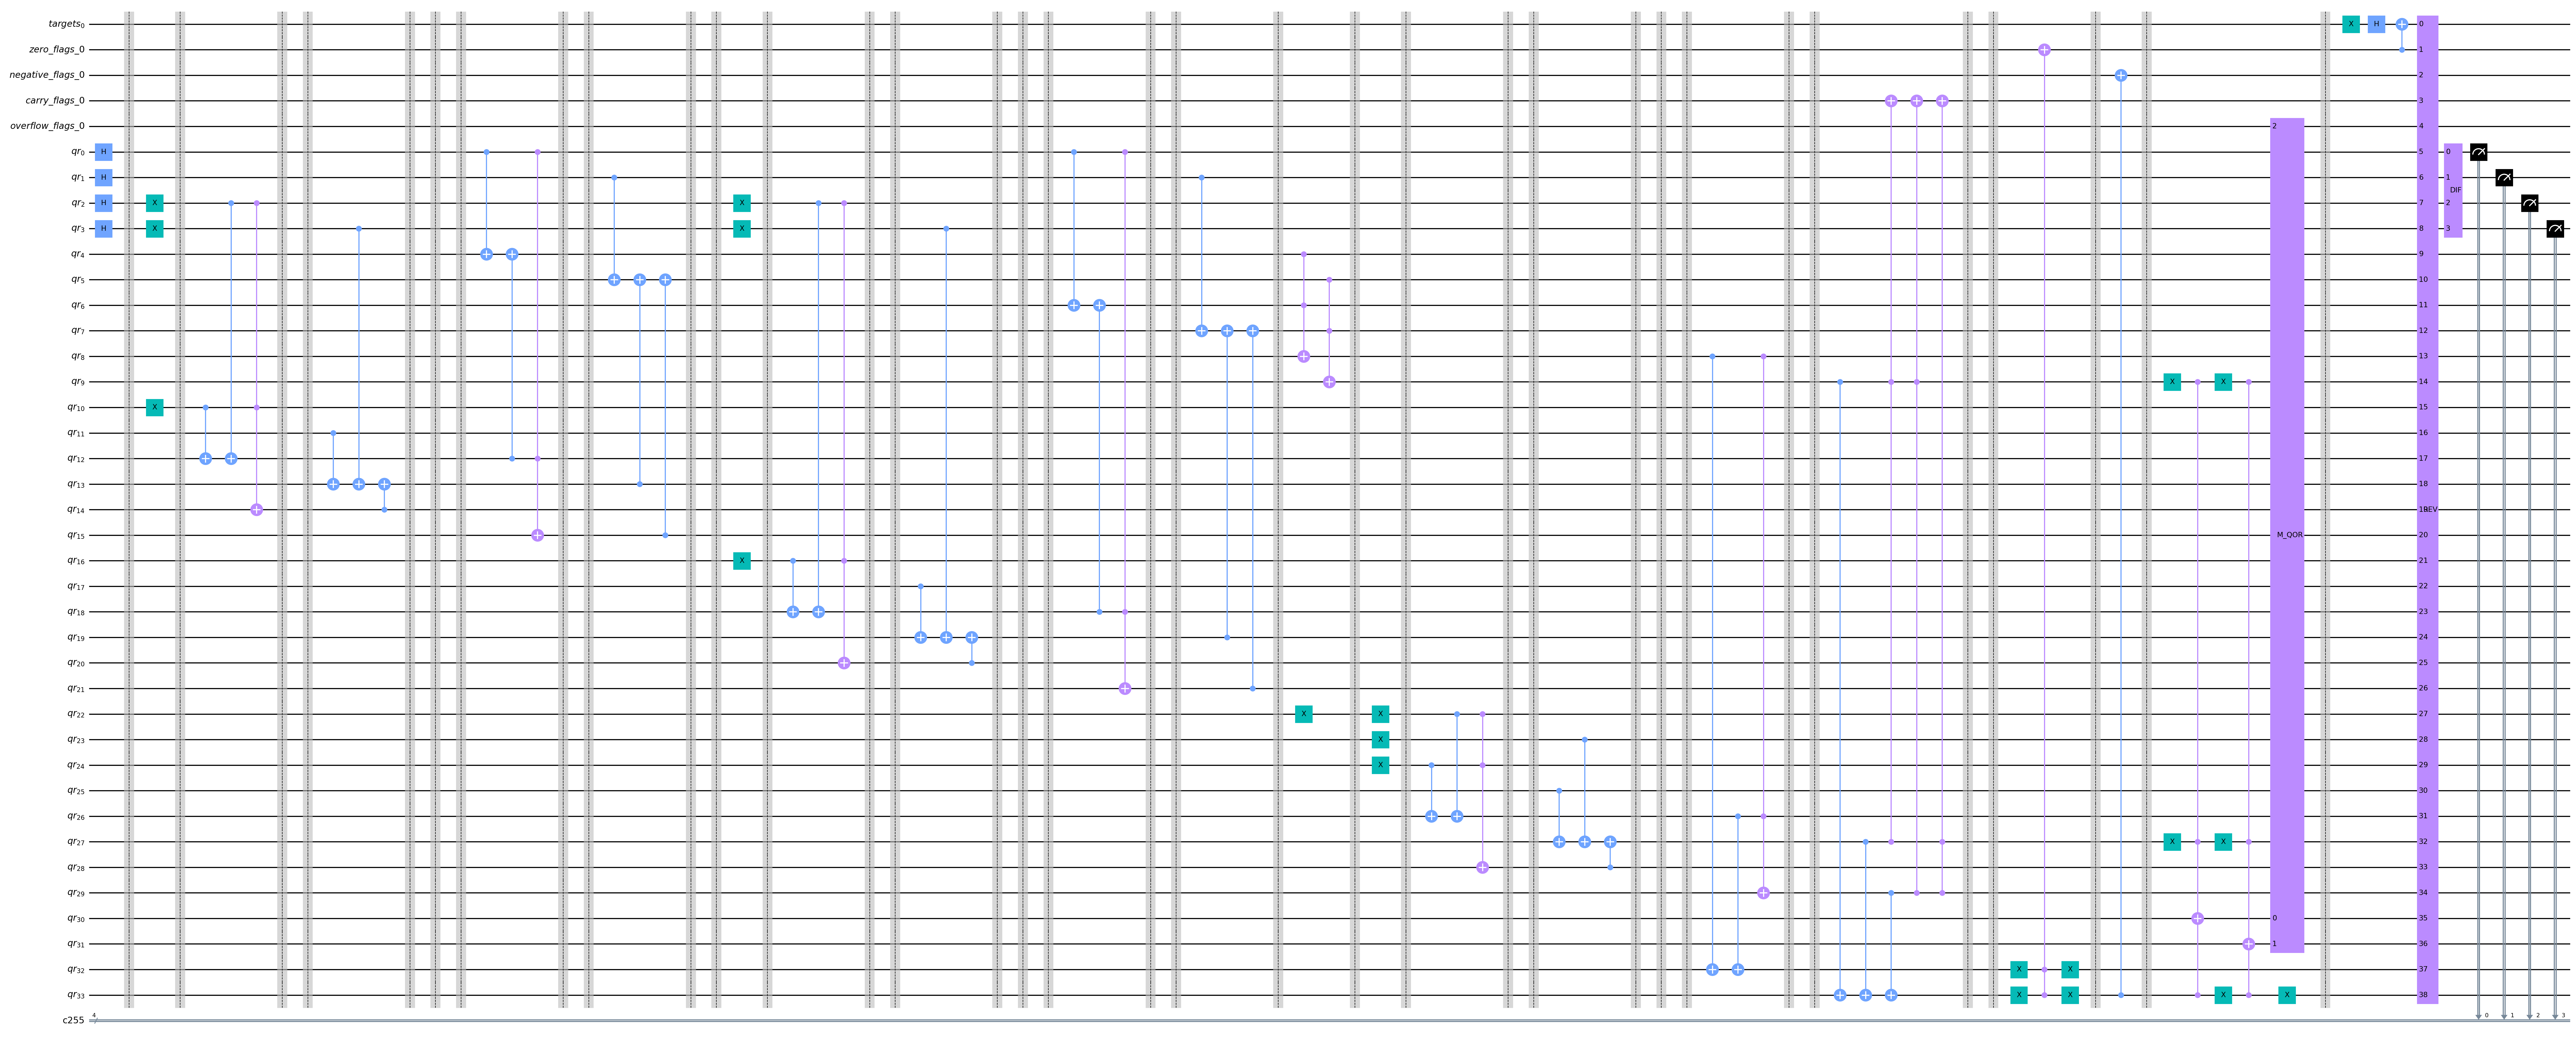
\includegraphics[width=9cm]{Figures/Minimum_Bisection_circuit.png}
    \caption{Using Grover's Algorithm to Solve the Minimum Bisection Problem}
    \label{fig:Minimum_Bisection}
\end{figure}

\section{Conclusion}

In this paper, we presented a novel approach to solving the Minimum Bisection problem using Grover's Algorithm. The proposed methodology leverages the quadratic speedup provided by Grover's Algorithm to efficiently search for an optimal solution to the problem. We transformed the Minimum Bisection problem into a decision problem, designed an oracle function to mark the solutions that satisfy the decision problem, and implemented the oracle as a quantum circuit. Performance analysis of the proposed approach demonstrated its potential to significantly outperform classical algorithms in solving the Minimum Bisection problem.

Our work contributes to the ongoing research in quantum computing and optimization by providing a practical application of Grover's Algorithm to a well-known NP-hard problem. This research not only showcases the potential of quantum computing in tackling challenging optimization problems but also paves the way for future studies exploring the application of quantum algorithms to other combinatorial optimization problems.

As quantum computing technology continues to advance, it is expected that larger problem instances and more complex optimization problems will become feasible for quantum-based solutions. Future work may focus on further optimizing the proposed approach, exploring the use of other quantum algorithms for solving the Minimum Bisection problem, and extending the methodology to handle different types of graph partitioning problems.

